\exercise[Robot Vision]

\subsection{Description of joint estimation algorithm}
The first step is to locate the joints in each of the camera feeds using
simple blob detection:
\begin{enumerate}
    \item
        For each joint, we threshold all pixels in the image to see
        which are in that joint's colour range.
    \item
        We then find the center of all thresholded pixels using
        OpenCV's \texttt{moments} function, giving us the location
        of this joint in the camera feed.
    \item
        We use the distance in pixels and metres between the yellow
        and blue blob to map all locations from pixels to metres.
\end{enumerate}
We then combine the 2D coordinates from both cameras to produce
estimates for the 3D joint locations. We make one very important
simplification: we compute the 3D locations as if the camera
gives a "bird's eye" view of each of the joints.
This is inherently inaccurate, and we could use ray casting in both camera feeds
to come up with more accurate 3D locations.\\
This simplification allows us to determine the coordinates for each joint:
\[ 
    J_i = \begin{bmatrix} x \\ y \\ z \end{bmatrix} =
    \begin{bmatrix} 
        \text{cam}_2.x \\
        \text{cam}_1.x \\
        \frac{1}{2} (\text{cam}_1.y + \text{cam}_2.y)
    \end{bmatrix} 
\]
Using the 3D estimates, we can compute the angles for each of the joints:
\begin{itemize}
    \item
        Let $\theta_2, \theta_3, \theta_4$ be
        "joint2", "joint3", "joint4", respectively.
    \item $\vec{BG} = J_2 - J_1$, $\vec{GR} = J_3 - J_2$
    \item $\theta_2 = \atantwo(\vec{BG}[2], \vec{BG}[1]) - \frac{\pi}{2}$,
        let $\vec{BG'}$ be $\vec{BG}$ rotated around the x-axis by $-\theta_2$
    \item $\theta_3 = \atantwo(\vec{BG'}[0], \vec{BG'}[2])$
    \item $\theta_4 = \atantwo(\vec{GR}[2],\vec{GR}[1]) - \theta_2 - \frac{\pi}{2}$
\end{itemize}

\subsection{Comparing estimations with sinusoidal signals}
\begin{center}
    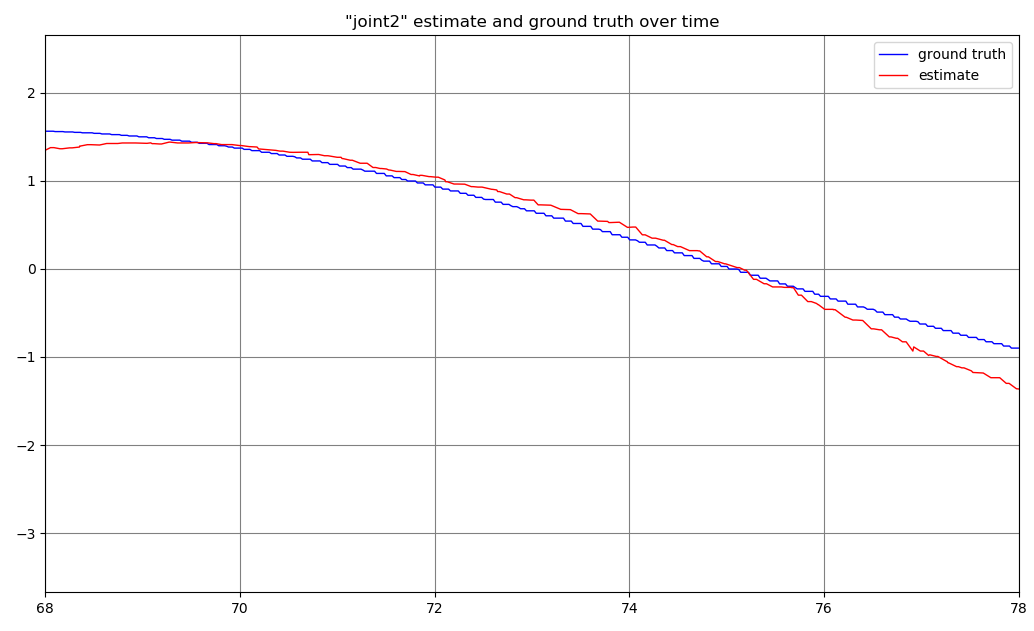
\includegraphics[width=0.7\textwidth]{plots/q2_1_j2_10sec.png}
    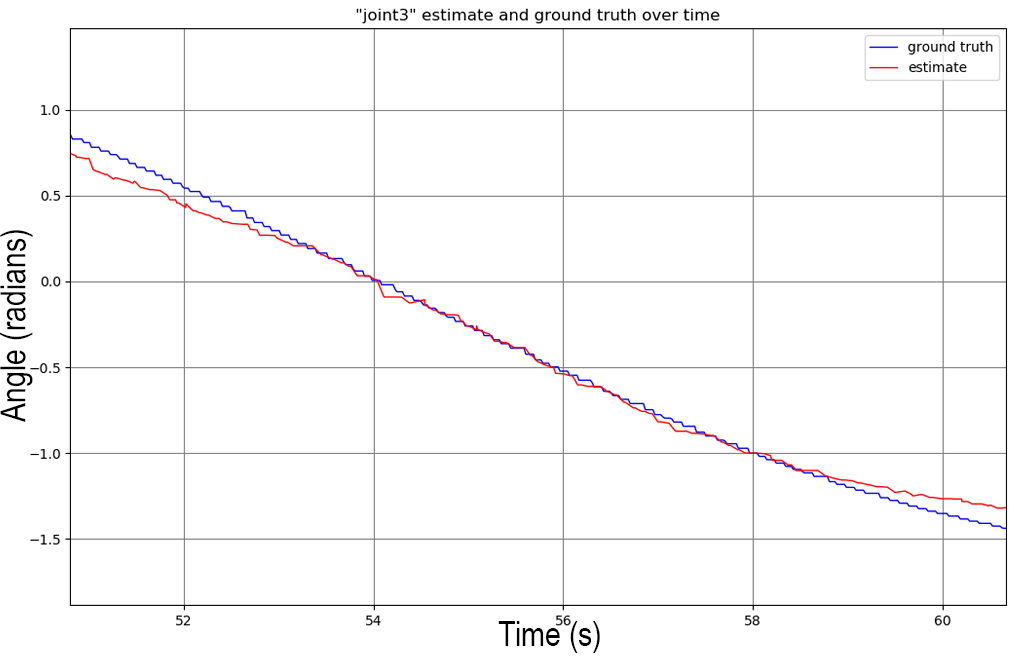
\includegraphics[width=0.7\textwidth]{plots/q2_1_j3_10sec.png}
    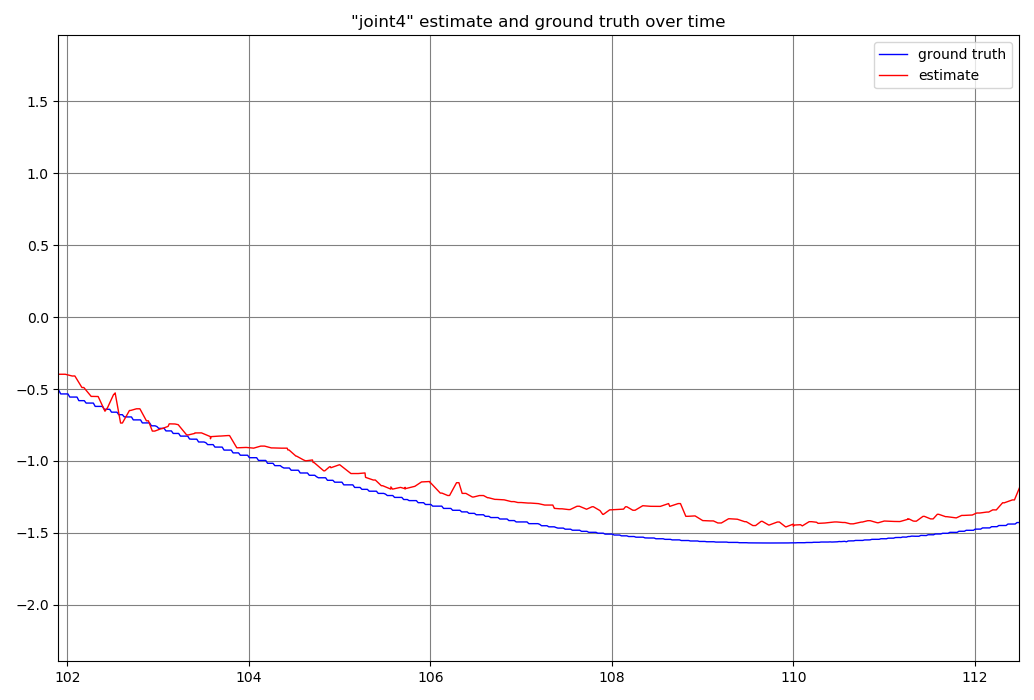
\includegraphics[width=0.7\textwidth]{plots/q2_1_j4_10sec.png}
\end{center}

\subsection{Description of target detection algorithm}
First, we detect the target in both of the camera feeds using 
template matching:
\begin{enumerate}
    \item \textbf{Isolate orange} elements using OpenCV's \texttt{inRange}
        method.
    \item 
        To distinguish between the target (sphere) and decoy
        (box), we perform \textbf{pattern matching} using OpenCV's
        \texttt{matchTemplate} method.
        We use a white circle with a darkened top and bottom
        so that the difference between the sphere and the box
        is more apparent.
    \item
        From the resulting image, we grab the position with the
        \textbf{least error} to determine the location of our target.
\end{enumerate}
Then, we combine both camera feeds to produce the 3D coordinates:
\begin{enumerate}
    \item
        Similar to the joints estimation algorithm, we assume that
        the camera feeds provide an orthogonal view across the
        entire plane.
    \item
        This simplification allows us to determine the coordinates:
        \[
            T = \begin{bmatrix} x \\ y \\ z \end{bmatrix} =
            \begin{bmatrix} 
                \text{cam}_2.x \\
                \text{cam}_1.x \\
                \frac{1}{2} (\text{cam}_1.y + \text{cam}_2.y)
            \end{bmatrix} 
        \]
\end{enumerate}

\subsection{Target detection plot}
\begin{center}
    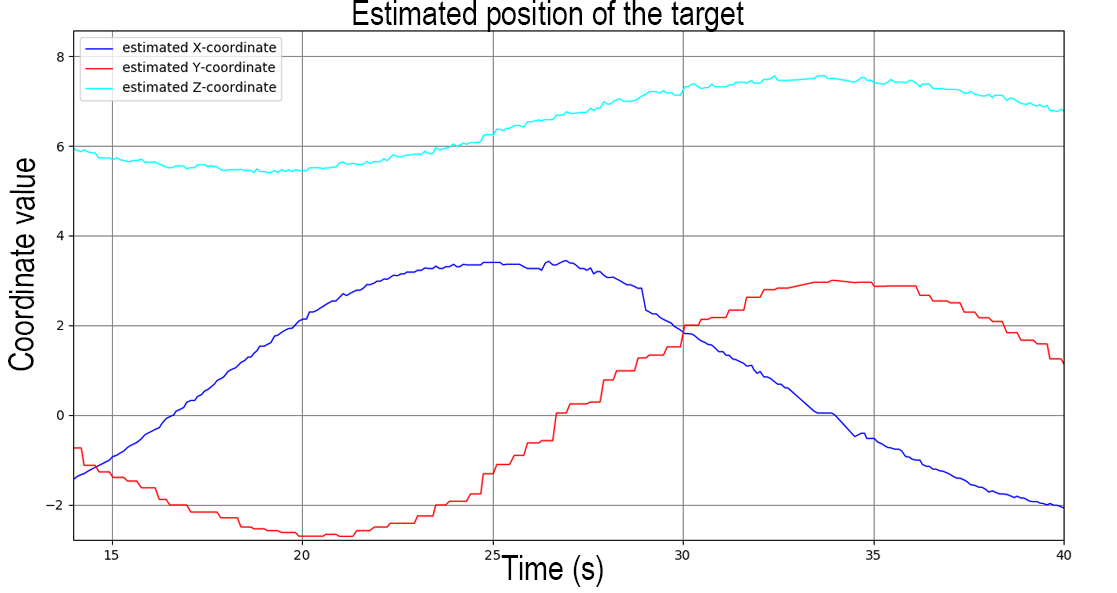
\includegraphics[width=0.8\textwidth]{plots/q2_2.png}
\end{center}
